\documentclass[12pt,letterpaper]{article}
\usepackage{graphicx,textcomp}
\usepackage{float}
\usepackage{natbib}
\usepackage{setspace}
\usepackage{fullpage}
\usepackage{color}
\usepackage[reqno]{amsmath}
\usepackage{amsthm}
\usepackage{fancyvrb}
\usepackage{amssymb,enumerate}
\usepackage[all]{xy}
\usepackage{endnotes}
\usepackage{lscape}
\newtheorem{com}{Comment}
\usepackage{float}
\usepackage{hyperref}
\newtheorem{lem} {Lemma}
\newtheorem{prop}{Proposition}
\newtheorem{thm}{Theorem}
\newtheorem{defn}{Definition}
\newtheorem{cor}{Corollary}
\newtheorem{obs}{Observation}
\usepackage[compact]{titlesec}
\usepackage{dcolumn}
\usepackage{tikz}
\usetikzlibrary{arrows}
\usepackage{multirow}
\usepackage{xcolor}
\usepackage{indentfirst}
\newcolumntype{.}{D{.}{.}{-1}}
\newcolumntype{d}[1]{D{.}{.}{#1}}
\definecolor{light-gray}{gray}{0.65}
\usepackage{url}
\usepackage{listings}
\usepackage{color}

\definecolor{codegreen}{rgb}{0,0.6,0}
\definecolor{codegray}{rgb}{0.5,0.5,0.5}
\definecolor{codepurple}{rgb}{0.58,0,0.82}
\definecolor{backcolour}{rgb}{0.95,0.95,0.92}

\lstdefinestyle{mystyle}{
	backgroundcolor=\color{backcolour},   
	commentstyle=\color{codegreen},
	keywordstyle=\color{magenta},
	numberstyle=\tiny\color{codegray},
	stringstyle=\color{codepurple},
	basicstyle=\footnotesize,
	breakatwhitespace=false,         
	breaklines=true,                 
	captionpos=b,                    
	keepspaces=true,                 
	numbers=left,                    
	numbersep=5pt,                  
	showspaces=false,                
	showstringspaces=false,
	showtabs=false,                  
	tabsize=2
}
\lstset{style=mystyle}
\newcommand{\Sref}[1]{Section~\ref{#1}}
\newtheorem{hyp}{Hypothesis}


\title{White Racial Atititudes and the Role of Union Membership}
\date{Due: April 18, 2026}
\author{Zahra Khan}

\begin{document}
	\maketitle
	\section*{Background}
	In this project, I am replicating the study, "Labor Unions and White Racial Politics" by Paul Frymer and Jacob M. Grumbach, published in the American Journal of Political Science. 
	In this article, the authors aim to understand the relationship between union membership and white American racial politics. Specifically, the authors develop a theory that is contextually and temporally bounded, arguing that white union members exhibit lower levels of racial resentment and greater support for legislation and policies that may benefit African Americans than their non-union counterparts. 
	
	White racial attitudes have been explored in the academic literature for many decades; however, the authors point out that the intersection between those attitudes and labor unionism remains underdeveloped. Labor unions have historically been central to the expression of white racial attitudes and politics, and have fluctuated throughout the twentieth and twenty-first centuries. The authors site many crucial moments in which white labor union members have been deeply intertwined with racial politics; for example, in the late nineteenth to early twentieth centuries, nativist movements thrived within labor unions, with many white unionists forming organizations such as the Asiatic Exclusion League and passing legislation such as the Chinese Exclusion Act of 1882 and the Johnson-Reed Immigration Act of 1924. However, the authors point out that during the New Deal era, union leadership formed many historically progressive alliances with Civil Rights organizations, and the CIO sought to mobilize black workers. Now, we are in an era in which labor union membership is the most diverse it's been, with high rates of African American and Latino union members. This newfound diversity, forged over decades of union activism, is a crucial reason to conduct this research. 

	
	\maketitle
	\section*{Methodology}
	
	This study primarily uses data from the Cooperative Congressional Election Study (CCES) and the Voter Study Group (VSG). The CCES Common Content data contain biannual samples of 30,000 respondents, which the study then uses to estimate cross-sectional relationships between union membership and attitudes with reasonable accuracy given the low rates of union membership generally. They also use panel data to estimate the within-subject effects of gaining union membership on racial attitudes. Further, this panel data, collected between 2010 and 2014, was surveyed in three panel waves in 2010, 2012, and 2014.  The VSG dataset is a panel of about 8,000 respondents who were surveyed both in the 2012 and 2016 election cycles.
	In both of these studies, respondents state their union membership, both current and past union membership, allowing the authors to account for and estimate decay. The two main questions in the first data set are: 
	
	(1) “The Irish, Italians, Jews, and many other minorities overcame prejudice and worked their way up. Blacks should do the same without any special favors.”
	(2) “Generations of slavery and discrimination have created conditions that make it difficult for Blacks to work their way out of the lower class” (reverse coded).
	
	In which they are measured on a 5-point Likert scale. Then they sum these responses and rescale the resentment index. The VSG data dataset in addition to the questions used above, also asks:
	
	(3) It’s really a matter of some people not trying hard enough; if blacks would only try harder, they could be just as well off as whites. 
	(4) “Over the past few years, blacks have gotten less than they deserve” (reverse coded).
	
	They have also replicated their analyses using data from the American National Election Study (ANES), which has the same four questions as the VSG but a much smaller sample size. 
	
	To measure union members' support for affirmative action policies, they use the question targeting affirmative action from both studies. 
	
	In the cross-sectional analysis, the authors adjust regression estimates for standard individual-level and contextual covariates such as gender and age, and use a matching design to pair similar union members with nonunion members to estimate differences in their racial attitudes. In the panel design, the question is whether changes in union membership are associated with changes in individuals' racial attitudes. 
	

\maketitle
\section*{Original Study}
The authors use OLS linear regression models to first determine whether union membership affects racial resentment. In addition, they test whether union membership would increase support for affirmative action policies benefiting African Americans, while controlling for Gender, Age, Education, and Income in both studies.


** Note that the authors include a table from running a matching estimator to compare similar individuals by union membership, which I was unable to replicate due to runtime constraints. 


\begin{table}[H]  \centering 
	\caption{Union Membership and Racial Resentment among Whites} 
	\label{Outcome: Racial Resentment} 
	\resizebox{\linewidth}{!}{
	\begin{tabular}{@{\extracolsep{5pt}}lccc} 
		\\[-1.8ex]\hline 
		\hline \\[-1.8ex] 
		& \multicolumn{3}{c}{\textit{Dependent variable:}} \\ 
		\cline{2-4} 
		\\[-1.8ex] & \multicolumn{3}{c}{Racial Resentment} \\ 
		\\[-1.8ex] & (1) & (2) & (3)\\ 
		\hline \\[-1.8ex] 
		Union Member & $-$0.063$^{***}$ & $-$0.047$^{***}$ & $-$0.048$^{***}$ \\ 
		& (0.005) & (0.005) & (0.005) \\ 
		& & & \\ 
		Past Union Member & $-$0.020$^{***}$ & $-$0.024$^{***}$ & $-$0.025$^{***}$ \\ 
		& (0.003) & (0.003) & (0.003) \\ 
		& & & \\ 
		Female &  & $-$0.046$^{***}$ & $-$0.046$^{***}$ \\ 
		&  & (0.002) & (0.002) \\ 
		& & & \\ 
		Income &  & 0.003$^{***}$ & 0.002$^{***}$ \\ 
		&  & (0.0004) & (0.0004) \\ 
		& & & \\ 
		Age &  & 0.0005$^{***}$ & 0.0005$^{***}$ \\ 
		&  & (0.0001) & (0.0001) \\ 
		& & & \\ 
		Education &  & $-$0.049$^{***}$ & $-$0.050$^{***}$ \\ 
		&  & (0.001) & (0.001) \\ 
		& & & \\ 
		Constant & 0.688$^{***}$ & 0.946$^{***}$ & 0.959$^{***}$ \\ 
		& (0.001) & (0.012) & (0.012) \\ 
		& & & \\ 
		\hline \\[-1.8ex] 
		State Fixed Effects & No & Yes & Yes \\ 
		Year Fixed Effects & No & No & Yes \\ 
		Observations & 71,431 & 61,463 & 61,463 \\ 
		R$^{2}$ & 0.003 & 0.080 & 0.081 \\ 
		Adjusted R$^{2}$ & 0.003 & 0.079 & 0.080 \\ 
		Residual Std. Error & 0.300 (df = 71428) & 0.288 (df = 61406) & 0.288 (df = 61405) \\ 
		F Statistic & 110.963$^{***}$ (df = 2; 71428) & 95.252$^{***}$ (df = 56; 61406) & 95.157$^{***}$ (df = 57; 61405) \\ 
		\hline 
		\hline \\[-1.8ex] 
		\textit{Note:}  & \multicolumn{3}{r}{$^{*}$p$<$0.1; $^{**}$p$<$0.05; $^{***}$p$<$0.01} \\ 
	\end{tabular} 
}
\lstinputlisting[language=R, firstline=97, lastline=99]{Labor_White_Racial_Politics_Code.R} 
Overall, this model found that union membership is associated with a reduction in racial resentment between 6.3 and 4.7\%, which is a significant result. In addition, past union membership is significantly and negatively associated with reduced racial resentment; however, the association is half that of current union members. 

\end{table} 


\begin{table}[H] \centering 
	\caption{VSG Panel Results of Union Membership and Racial Resentment among Whites} 
	\label{} 
	\resizebox{\linewidth}{!}{
	\begin{tabular}{@{\extracolsep{5pt}}lcccc} 
		\\[-1.8ex]\hline 
		\hline \\[-1.8ex] 
		& \multicolumn{4}{c}{\textit{Dependent variable:}} \\ 
		\cline{2-5} 
		\\[-1.8ex] & Racial Resentment 2016 & Racial Resentment Change & Racial Resentment 2016 & Racial Resentment Change \\ 
		\\[-1.8ex] & (1) & (2) & (3) & (4)\\ 
		\hline \\[-1.8ex] 
		Union Membership Gained & $-$0.046$^{***}$ & $-$0.044$^{***}$ & $-$0.048$^{***}$ & $-$0.046$^{***}$ \\ 
		& (0.015) & (0.015) & (0.015) & (0.015) \\ 
		& & & & \\ 
		Union Membership Lost & $-$0.010 & $-$0.010 & $-$0.007 & $-$0.007 \\ 
		& (0.015) & (0.015) & (0.015) & (0.016) \\ 
		& & & & \\ 
		Racial Resentment (t-1) & 0.930$^{***}$ &  & 0.906$^{***}$ &  \\ 
		& (0.010) &  & (0.011) &  \\ 
		& & & & \\ 
		Income &  &  & $-$0.0004 & $-$0.001 \\ 
		&  &  & (0.001) & (0.001) \\ 
		& & & & \\ 
		Female &  &  & $-$0.015$^{***}$ & $-$0.013$^{**}$ \\ 
		&  &  & (0.005) & (0.005) \\ 
		& & & & \\ 
		Education &  &  & $-$0.010$^{***}$ & $-$0.006$^{***}$ \\ 
		&  &  & (0.002) & (0.002) \\ 
		& & & & \\ 
		Age &  &  & 0.001$^{***}$ & 0.001$^{***}$ \\ 
		&  &  & (0.0002) & (0.0002) \\ 
		& & & & \\ 
		Constant & 0.007 & $-$0.034$^{***}$ & 0.027 & $-$0.041$^{***}$ \\ 
		& (0.006) & (0.002) & (0.017) & (0.015) \\ 
		& & & & \\ 
		\hline \\[-1.8ex] 
		Observations & 4,276 & 4,276 & 4,068 & 4,068 \\ 
		R$^{2}$ & 0.671 & 0.002 & 0.674 & 0.013 \\ 
		Adjusted R$^{2}$ & 0.671 & 0.002 & 0.674 & 0.011 \\ 
		Residual Std. Error & 0.154 (df = 4272) & 0.155 (df = 4273) & 0.153 (df = 4060) & 0.155 (df = 4061) \\ 
		F Statistic & 2,902.799$^{***}$ (df = 3; 4272) & 4.668$^{***}$ (df = 2; 4273) & 1,201.116$^{***}$ (df = 7; 4060) & 8.595$^{***}$ (df = 6; 4061) \\ 
		\hline 
		\hline \\[-1.8ex] 
		\textit{Note:}  & \multicolumn{4}{r}{$^{*}$p$<$0.1; $^{**}$p$<$0.05; $^{***}$p$<$0.01} \\ 
	\end{tabular} 
}
\lstinputlisting[language=R, firstline=557, lastline=562]{Labor_White_Racial_Politics_Code.R} 
note* table 2 and 3 are apart of the same model, however I was unable to run the tables together with stargazer. 
The effect of becoming a union member across the model from 2010 to 2016 is a reduction of racial resentment of about 4.1 and 4.8\% in the resentment index. However, compared to the previous model, losing union membership is unrelated to racial resentment. 
\end{table}

\begin{table}[H] \centering 
	\caption{VSG Panel Results of Union Membership and Racial Resentment among Whites} 
	\label{} 
	\resizebox{\linewidth}{!}{
	\begin{tabular}{@{\extracolsep{5pt}}lcc} 
		\\[-1.8ex]\hline 
		\hline \\[-1.8ex] 
		& \multicolumn{2}{c}{\textit{Dependent variable:}} \\ 
		\cline{2-3} 
		\\[-1.8ex] & Racial Resentment 2016 & Racial Resentment Change  \\ 
		\\[-1.8ex] & (1) & (2)\\ 
		\hline \\[-1.8ex] 
		Union Membership Gained & $-$0.042$^{***}$ & $-$0.041$^{***}$ \\ 
		& (0.015) & (0.015) \\ 
		& & \\ 
		Union Membership Lost & $-$0.003 & 0.0003 \\ 
		& (0.015) & (0.015) \\ 
		& & \\ 
		Racial Resentment (t-1) &  & 0.813$^{***}$ \\ 
		&  & (0.012) \\ 
		& & \\ 
		Party ID & $-$0.055$^{***}$ & $-$0.115$^{***}$ \\ 
		& (0.007) & (0.008) \\ 
		& & \\ 
		Income & $-$0.001 & $-$0.001 \\ 
		& (0.001) & (0.001) \\ 
		& & \\ 
		Female & $-$0.007 & $-$0.007 \\ 
		& (0.005) & (0.005) \\ 
		& & \\ 
		Education & $-$0.005$^{***}$ & $-$0.011$^{***}$ \\ 
		& (0.002) & (0.002) \\ 
		& & \\ 
		Age & 0.001$^{***}$ & 0.001$^{***}$ \\ 
		& (0.0002) & (0.0002) \\ 
		& & \\ 
		Constant & $-$0.019 & 0.143$^{***}$ \\ 
		& (0.015) & (0.018) \\ 
		& & \\ 
		\hline \\[-1.8ex] 
		Observations & 3,994 & 3,994 \\ 
		R$^{2}$ & 0.029 & 0.693 \\ 
		Adjusted R$^{2}$ & 0.027 & 0.692 \\ 
		Residual Std. Error & 0.153 (df = 3986) & 0.149 (df = 3985) \\ 
		F Statistic & 17.041$^{***}$ (df = 7; 3986) & 1,124.111$^{***}$ (df = 8; 3985) \\ 
		\hline 
		\hline \\[-1.8ex] 
		\textit{Note:}  & \multicolumn{2}{r}{$^{*}$p$<$0.1; $^{**}$p$<$0.05; $^{***}$p$<$0.01} \\ 
	\end{tabular} 
}
\end{table} 

\begin{table}[H] \centering 
	\caption{ CCES Panel Results of Union Membership and Racial Resentment among Whites} 
	\label{} 
	\resizebox{\linewidth}{!}{
		\begin{tabular}{@{\extracolsep{5pt}}lcccc} 
			\\[-1.8ex]\hline \\[-1.8ex] 
			\\[-1.8ex] & \multicolumn{4}{c}{\textbf{Outcome: Racial Resentment}} \\ 
			\\[-1.8ex] & \textbf{Model 1} & \textbf{Model 2} & \textbf{Model 3} & \textbf{Model 4}\\ 
			\hline \\[-1.8ex] 
			Gained Union Membership & $-$0.055$^{***}$ & $-$0.055$^{***}$ & $-$0.051$^{***}$ & $-$0.049$^{***}$ \\ 
			& (0.018) & (0.018) & (0.019) & (0.018) \\ 
			Lost Union Membership & 0.0002 & $-$0.00001 & $-$0.003 & 0.009 \\ 
			& (0.032) & (0.032) & (0.033) & (0.033) \\ 
			Racial Resentment (t-1) & 0.899$^{***}$ & 0.899$^{***}$ & 0.884$^{***}$ & 0.797$^{***}$ \\ 
			& (0.005) & (0.005) & (0.005) & (0.007) \\ 
			Party ID (Democratic) &  &  &  & $-$0.124$^{***}$ \\ 
			&  &  &  & (0.005) \\ 
			Income &  &  & 0.0004 & $-$0.0005 \\ 
			&  &  & (0.001) & (0.001) \\ 
			Female &  &  & $-$0.007$^{*}$ & 0.002 \\ 
			&  &  & (0.003) & (0.003) \\ 
			Age &  &  & 0.0003$^{**}$ & 0.0002 \\ 
			&  &  & (0.0001) & (0.0001) \\ 
			Education &  &  & $-$0.010$^{***}$ & $-$0.010$^{***}$ \\ 
			&  &  & (0.001) & (0.001) \\ 
			Constant & 0.056$^{***}$ & 0.054$^{***}$ & 0.084$^{***}$ & 0.215$^{***}$ \\ 
			& (0.004) & (0.004) & (0.012) & (0.014) \\ 
			Year Fixed Effects & No & Yes & Yes & Yes \\ 
			N & 10908 & 10908 & 9726 & 9617 \\ 
			R-squared & 0.749 & 0.749 & 0.749 & 0.764 \\ 
			Adj. R-squared & 0.749 & 0.749 & 0.749 & 0.764 \\ 
			Residual Std. Error & 0.165 (df = 10904) & 0.165 (df = 10903) & 0.165 (df = 9717) & 0.161 (df = 9607) \\ 
			F Statistic & 10863.440$^{***}$ (df = 3; 10904) & 8148.794$^{***}$ (df = 4; 10903) & 3629.656$^{***}$ (df = 8; 9717) & 3454.658$^{***}$ (df = 9; 9607) \\ 
			\hline \\[-1.8ex] 
			\multicolumn{5}{l}{$^{***}$p $<$ .01; $^{**}$p $<$ .05; $^{*}$p $<$ .1} \\ 
		\end{tabular} 
	}
	\lstinputlisting[language=R, firstline=39, lastline=42]{Labor_White_Racial_Politics_Code.R}
	 This model shows that, although slightly larger, the effect is similar, ranging from -0.049 to 0.055 in reducing racial resentment over time. In addition, once again, the loss of membership has an insignificant effect on racial resentment.
	 
\end{table} 


\begin{table}[H] \centering 
	\caption{Union Membership and White Support for Policies That Benefit African Americans} 
	\label{} 
	\begin{tabular}{@{\extracolsep{5pt}}lccc} 
		\\[-1.8ex]\hline 
		\hline \\[-1.8ex] 
		& \multicolumn{3}{c}{\textit{Dependent variable:}} \\ 
		\cline{2-4} 
		\\[-1.8ex] & \multicolumn{3}{c}{ Racial Policy Index} \\ 
		\\[-1.8ex] & (1) & (2) & (3)\\ 
		\hline \\[-1.8ex] 
		Union Membership & 0.036$^{**}$ & 0.041$^{**}$ & 0.040$^{**}$ \\ 
		& (0.018) & (0.018) & (0.018) \\ 
		& & & \\ 
		Sex &  & 0.014 & 0.014 \\ 
		&  & (0.011) & (0.011) \\ 
		& & & \\ 
		Age &  & $-$0.0002 & $-$0.0002 \\ 
		&  & (0.0003) & (0.0003) \\ 
		& & & \\ 
		Income &  & $-$0.048$^{***}$ & $-$0.048$^{***}$ \\ 
		&  & (0.005) & (0.005) \\ 
		& & & \\ 
		Education &  & 0.029$^{***}$ & 0.029$^{***}$ \\ 
		&  & (0.004) & (0.004) \\ 
		& & & \\ 
		Constant & 0.301$^{***}$ & 0.341$^{***}$ & 0.331$^{***}$ \\ 
		& (0.006) & (0.031) & (0.032) \\ 
		& & & \\ 
		\hline \\[-1.8ex] 
		Region Fixed Effects & No & Yes & Yes \\ 
		Year Fixed Effects & No & No & Yes \\ 
		Observations & 2,650 & 2,431 & 2,431 \\ 
		R$^{2}$ & 0.002 & 0.052 & 0.053 \\ 
		Adjusted R$^{2}$ & 0.001 & 0.048 & 0.049 \\ 
		Residual Std. Error & 0.279 (df = 2648) & 0.273 (df = 2422) & 0.273 (df = 2418) \\ 
		F Statistic & 4.116$^{**}$ (df = 1; 2648) & 16.440$^{***}$ (df = 8; 2422) & 11.342$^{***}$ (df = 12; 2418) \\ 
		\hline 
		\hline \\[-1.8ex] 
		\textit{Note:}  & \multicolumn{3}{r}{$^{*}$p$<$0.1; $^{**}$p$<$0.05; $^{***}$p$<$0.01} \\ 
	\end{tabular} 
\lstinputlisting[language=R, firstline=173, lastline=175]{Labor_White_Racial_Politics_Code.R} 
The coefficient estimates are between 0.036 and 0.041, which indicates that union membership is positively associated with supporting affirmative action policies.
\end{table} 

In both panel and cross-sectional models, union membership and gaining union membership is consistently associated with a substantial reduction in racial resentment. In addition, as shown in the last figure, union membership is positively associated with support for affirmative action policies that benefit African Americans. When interpreting these results as a whole, we conclude that union membership has a significant impact on white racial politics, in ways the authors anticipated based on existing histories and theories. 



\newpage
\maketitle
\section*{Adding an Interaction Term}

I chose to test whether there is an interaction between Union Membership and Age. First, I hypothesized that there is an interaction between Union Membership and Age, in which Union Membership would have a negative effect on the association between Age and Racial Resentment. This hypothesis is rooted in an extensive and complex history of racism amongst labor unions throughout the greater portion of the twentieth century. This history begins in the early twentieth century with the development of the Asiatic Exclusion League and its aim of pushing for Chinese Exclusion. Further, into the eighties, labor unions were crucial actors in rallying support for the 1986 Immigration Reform and Control Act, which targeted Mexican and Central American immigrants. However, alongside this problematic history, labor unions have often aligned with the Democratic Party and organized alongside marginalized groups, especially in times of need. Given this complicated history, I was initially unsure what the association would be. Prior to running the model, I first binned and factored the age variable for both the cross-sectional and panel data models on the CCES studies. For the cross-sectional model, I also created an interflux plot to illustrate my findings.


Sources for Historical Context:
Chavex, Leo R. Immigration Reform and Nativism: The Nationalist Response to the Transnationalist Challenge. Blackwell Publishing 2003.

Disalvo, Daniel. “The Politics of a Party Faction: The LiberalLabor Alliance in the Democratic Party,
1948–1972”  The Journal of Policy History (2010).

Gendzel, Glen. “It Didn It Didn’t Start Start with Proposition 187: One Hundred and Fifty Years of Nativist Legislation in California” Journal of the West (2009): 76-85.

For the Cross-Sectional
\lstinputlisting[language=R, firstline=115, lastline=123]{Labor_White_Racial_Politics_Code.R} 
For the Panel:
\lstinputlisting[language=R, firstline=80, lastline=83]{Labor_White_Racial_Politics_Code.R} 
\newpage	

\begin{table}[H] \centering 
	\caption{} 
	\label{} 
		\resizebox{\linewidth}{!}{
	\begin{tabular}{@{\extracolsep{5pt}}lccc} 
		\\[-1.8ex]\hline 
		\hline \\[-1.8ex] 
		& \multicolumn{3}{c}{\textit{Dependent variable:}} \\ 
		\cline{2-4} 
		\\[-1.8ex] & \multicolumn{3}{c}{racial resentment} \\ 
		\\[-1.8ex] & (1) & (2) & (3)\\ 
		\hline \\[-1.8ex] 
		union member & $-$0.063$^{***}$ & $-$0.013 & $-$0.014 \\ 
		& (0.005) & (0.018) & (0.018) \\ 
		& & & \\ 
		past union member & $-$0.020$^{***}$ & $-$0.025$^{***}$ & $-$0.025$^{***}$ \\ 
		& (0.003) & (0.003) & (0.003) \\ 
		& & & \\ 
		Female &  & $-$0.046$^{***}$ & $-$0.045$^{***}$ \\ 
		&  & (0.002) & (0.002) \\ 
		& & & \\ 
		Income &  & 0.002$^{***}$ & 0.002$^{***}$ \\ 
		&  & (0.0004) & (0.0004) \\ 
		& & & \\ 
		age 31-50 &  & 0.059$^{***}$ & 0.057$^{***}$ \\ 
		&  & (0.005) & (0.005) \\ 
		& & & \\ 
		age 51-70 &  & 0.052$^{***}$ & 0.051$^{***}$ \\ 
		&  & (0.004) & (0.004) \\ 
		& & & \\ 
		age\_binned 70+ &  & 0.042$^{***}$ & 0.042$^{***}$ \\ 
		&  & (0.005) & (0.005) \\ 
		& & & \\ 
		Education &  & $-$0.049$^{***}$ & $-$0.049$^{***}$ \\ 
		&  & (0.001) & (0.001) \\ 
		& & & \\ 
		union member: age 31-50 &  & $-$0.004 & $-$0.003 \\ 
		&  & (0.020) & (0.020) \\ 
		& & & \\ 
		union member: age 51-70 &  & $-$0.051$^{***}$ & $-$0.050$^{***}$ \\ 
		&  & (0.019) & (0.019) \\ 
		& & & \\ 
		union member:age 70+ &  & $-$0.083$^{***}$ & $-$0.082$^{***}$ \\ 
		&  & (0.026) & (0.026) \\ 
		& & & \\ 
		Constant & 0.688$^{***}$ & 0.926$^{***}$ & 0.940$^{***}$ \\ 
		& (0.001) & (0.012) & (0.012) \\ 
		& & & \\ 
		\hline \\[-1.8ex] 
		State Fixed Effects & No & Yes & Yes \\ 
		Year Fixed Effects & No & No & Yes \\ 
		Observations & 71,431 & 61,463 & 61,463 \\ 
		R$^{2}$ & 0.003 & 0.083 & 0.084 \\ 
		Adjusted R$^{2}$ & 0.003 & 0.082 & 0.083 \\ 
		Residual Std. Error & 0.300 (df = 71428) & 0.288 (df = 61401) & 0.287 (df = 61400) \\ 
		F Statistic & 110.963$^{***}$ (df = 2; 71428) & 90.771$^{***}$ (df = 61; 61401) & 90.471$^{***}$ (df = 62; 61400) \\ 
		\hline 
		\hline \\[-1.8ex] 
		\textit{Note:}  & \multicolumn{3}{r}{$^{*}$p$<$0.1; $^{**}$p$<$0.05; $^{***}$p$<$0.01} \\ 
	\end{tabular} 
}
\end{table}

The first crucial observation is that, for the baseline category "18-35," the result is not statistically significant, indicating that, among younger members, union membership has no significant effect on racial resentment. 
Ages 31-50: For this interaction term, the interaction is not significantly different from zero, indicating statistical non-significance. However, for members ages 51-70, 0.052 - 0.051 = 0.001, indicating that union membership almost completely cancels out the effect of age on racial resentment. Further, for members over the age of seventy, union membership can cancel out the effect of age on racial resentment altogether and push older members below the baseline 0.042 - 0.082 = -0.041.


\begin{figure}[H]
	\centering
	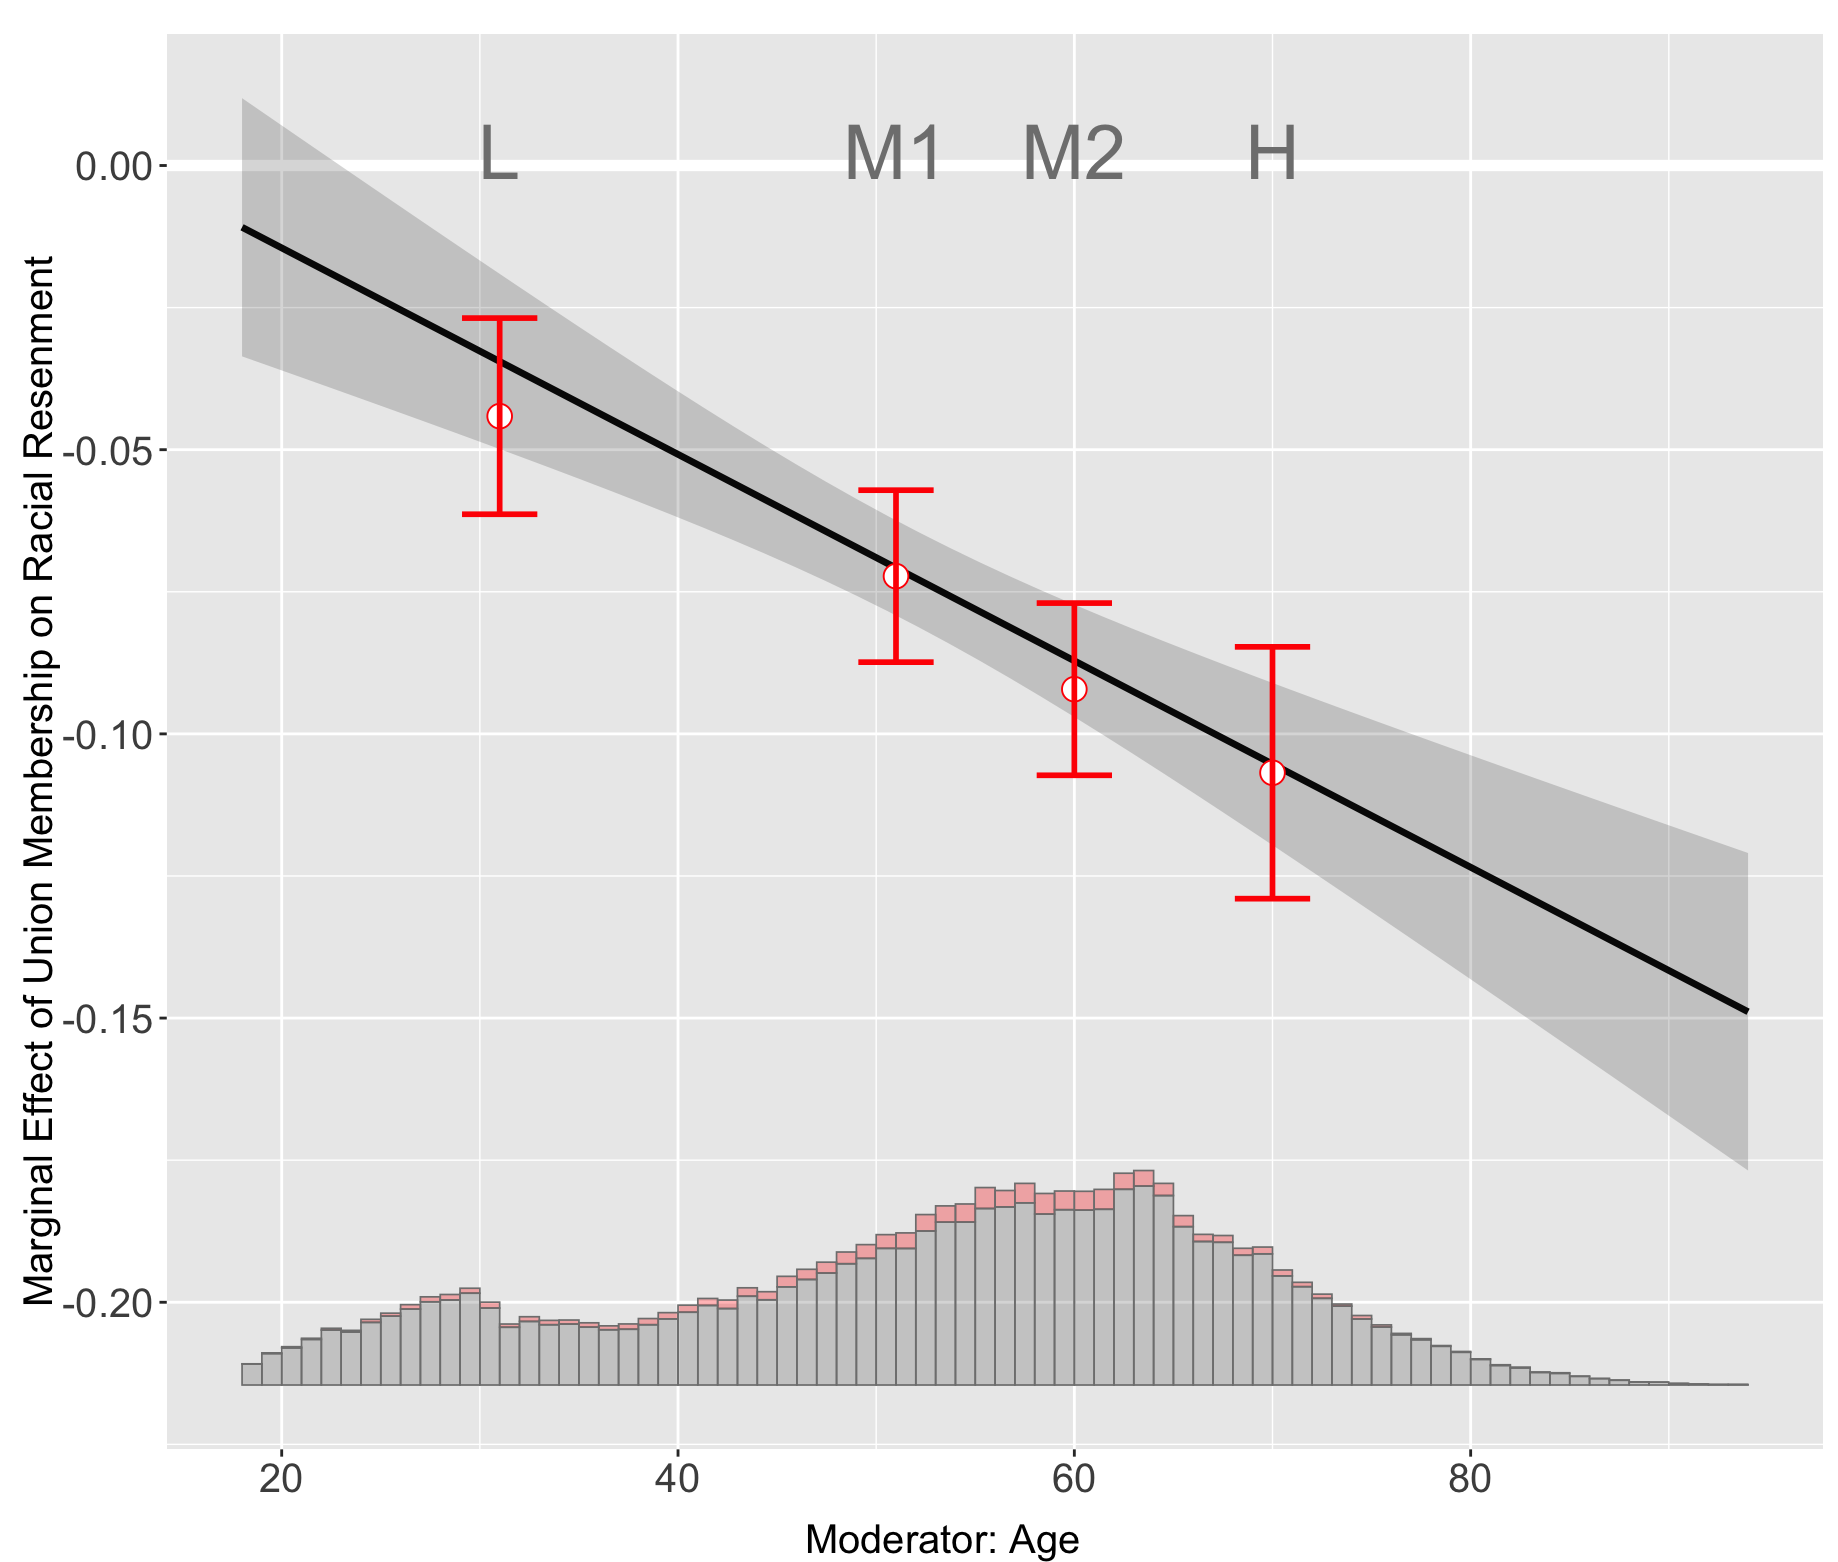
\includegraphics[width=10cm]{Interflux.png}
	\label{fig:Interflux Graph}
\end{figure}
This graph shows that the effect of union membership on racial resentment becomes more negative as one ages. Unions are more strongly associated with reduced racial resentment among older members than among younger ones. 
Further, the red points are the estimated marginal effects for the age bins with 95\% confidence intervals. Finally, the histogram at the bottom shows the distribution of respondents' ages, indicating that most are around 50-65 years old, which may have skewed the results. 
\lstinputlisting[language=R, firstline=136, lastline=147]{Labor_White_Racial_Politics_Code.R}  
\vspace{0.01cm}
\begin{table}[H] \centering 
	\caption{} 
	\label{} 
		\resizebox{\linewidth}{!}{
	\begin{tabular}{@{\extracolsep{5pt}}lcccc} 
		\\[-1.8ex]\hline \\[-1.8ex] 
		\\[-1.8ex] & \multicolumn{4}{c}{\textbf{racial\_resentment}} \\ 
		\\[-1.8ex] & \textbf{Model 1} & \textbf{Model 2} & \textbf{Model 3} & \textbf{Model 4}\\ 
		\hline \\[-1.8ex] 
		union\_gained & $-$0.055$^{***}$ & $-$0.055$^{***}$ & $-$0.048$^{*}$ & $-$0.041 \\ 
		& (0.018) & (0.018) & (0.028) & (0.028) \\ 
		union\_lost & 0.0002 & $-$0.00001 & $-$0.004 & 0.008 \\ 
		& (0.032) & (0.032) & (0.033) & (0.033) \\ 
		racial\_resentment\_lag & 0.899$^{***}$ & 0.899$^{***}$ & 0.884$^{***}$ & 0.795$^{***}$ \\ 
		& (0.005) & (0.005) & (0.006) & (0.007) \\ 
		dem\_id\_2010 &  &  &  & $-$0.125$^{***}$ \\ 
		&  &  &  & (0.006) \\ 
		faminc\_10 &  &  & 0.0004 & $-$0.001 \\ 
		&  &  & (0.001) & (0.001) \\ 
		factor(gender\_10)1 &  &  & $-$0.007$^{**}$ & 0.002 \\ 
		&  &  & (0.004) & (0.003) \\ 
		age\_factorg[60,80) &  &  & $-$0.005 & $-$0.004 \\ 
		&  &  & (0.004) & (0.004) \\ 
		age\_factorg[80,100] &  &  & 0.004 & $-$0.005 \\ 
		&  &  & (0.007) & (0.007) \\ 
		educ\_10 &  &  & $-$0.010$^{***}$ & $-$0.010$^{***}$ \\ 
		&  &  & (0.001) & (0.001) \\ 
		union\_gained:age\_factorg[60,80) &  &  & $-$0.007 & $-$0.007 \\ 
		&  &  & (0.040) & (0.039) \\ 
		union\_gained:age\_factorg[80,100] &  &  & $-$0.003 & $-$0.0003 \\ 
		&  &  & (0.167) & (0.162) \\ 
		Constant & 0.056$^{***}$ & 0.054$^{***}$ & 0.108$^{***}$ & 0.234$^{***}$ \\ 
		& (0.004) & (0.004) & (0.009) & (0.010) \\ 
		Year Fixed Effects & No & Yes & Yes & Yes \\ 
		N & 10908 & 10908 & 9333 & 9228 \\ 
		R-squared & 0.749 & 0.749 & 0.750 & 0.765 \\ 
		Adj. R-squared & 0.749 & 0.749 & 0.749 & 0.765 \\ 
		Residual Std. Error & 0.165 (df = 10904) & 0.165 (df = 10903) & 0.164 (df = 9321) & 0.160 (df = 9215) \\ 
		F Statistic & 10863.440$^{***}$ (df = 3; 10904) & 8148.794$^{***}$ (df = 4; 10903) & 2539.181$^{***}$ (df = 11; 9321) & 2497.975$^{***}$ (df = 12; 9215) \\ 
		\hline \\[-1.8ex] 
		\multicolumn{5}{l}{$^{***}$p $<$ .01; $^{**}$p $<$ .05; $^{*}$p $<$ .1} \\ 
	\end{tabular} 
}

\end{table} 
After running the panel data with the interaction term, I found that, as with the additive model, the interaction term between Union Membership and Racial Resentment is not statistically significant. A possible reason for the lack of significance could be that, as respondents age, their opinions do not change meaningfully; the within-person variation attributable to aging over time is either very small or null in 2010 and 2014. Further, factoring in age does not yield any statistically significant age groups. 

\end{document}
 